\documentclass[border=10pt]{standalone}
\usepackage{pgfplots}
\pgfplotsset{compat=1.18}
\usepackage{tikz}

\begin{document}
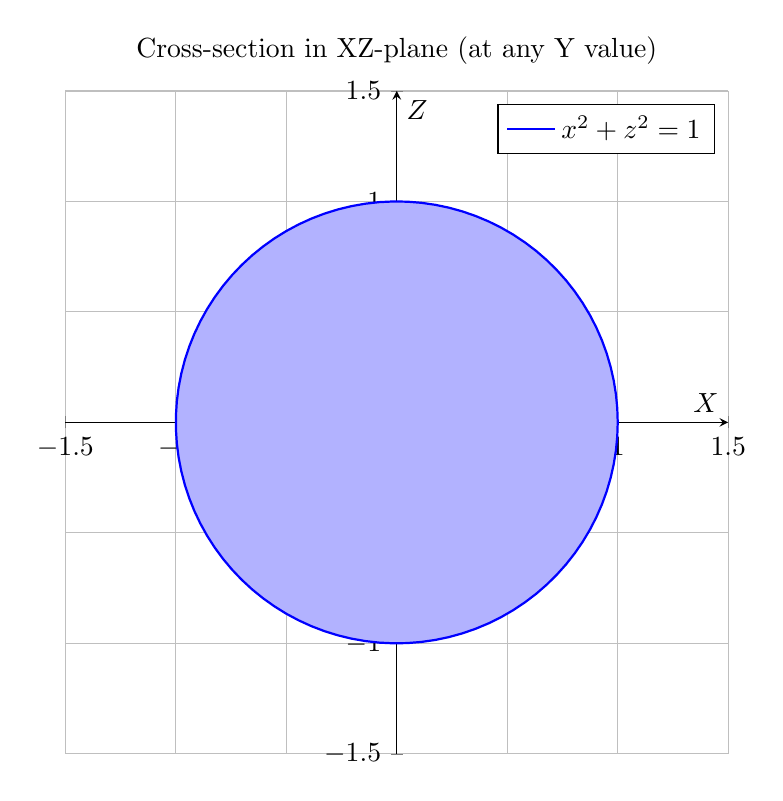
\begin{tikzpicture}
\begin{axis}[
    width=10cm,
    height=10cm,
    xlabel=$X$,
    ylabel=$Z$,
    title={Cross-section in XZ-plane (at any Y value)},
    axis lines=center,
    grid=major,
    axis equal,
    xmin=-1.5, xmax=1.5,
    ymin=-1.5, ymax=1.5,
]
    % Draw the unit circle
    \addplot[domain=0:360, samples=100, blue, thick, fill=blue!30] ({cos(x)}, {sin(x)});
    \addlegendentry{$x^2 + z^2 = 1$}
\end{axis}
\end{tikzpicture}
\end{document}